% !TEX encoding = UTF-8 Unicode
\documentclass[12pt]{article}

% Pacotes %
\usepackage[brazilian]{babel}
\usepackage[utf8]{inputenc}
\usepackage[T1]{fontenc}
\usepackage{amsmath}
\usepackage{enumitem}
\usepackage{hyperref}
\usepackage{graphicx}
\usepackage{verbatimbox}
\usepackage{ esint }
\usepackage[margin=1in]{geometry}

% Definições de titulo e autores %
\title{CI164\\Iniciação à Computação Científica\\Trabalho 2}
\author{
	Giancarlo Klemm Camilo \\
	Renan Domingos Merlin Greca
}
\date{Junho de 2015}

% Inicio do documento %
\begin{document}

% ------------------------------------------------------ %
% Página inicial %
\maketitle
\newpage	

% ------------------------------------------------------ %
% Indice %
\tableofcontents
\newpage

% ------------------------------------------------------ %
\section{Introdução}
O objetivo deste trabalho é a implementação de programa para resolver o PDE:
\begin{align*}
	- \Delta u(x,y) + k^2u(x,y) &= \fint (x,y),	(x,y) \in \Omega\\
	\fint(x,y) &= 4 \pi sin(2 \pi x) sinh(2 \pi y) \\
	\Omega &= [0,2] \times [0,1] \\
	u(x,1) &= sin(2 \pi x) sinh(2 \pi) \\
	u(x,0) &= u(0,y) = u(2,y) = 0
\end{align*}

Após o programa inicial foi feito, várias alterações foram feitas para melhorar o desempenho.
Os métodos utilizados para análise do código, sistema de testes, otimizações de código e de estruturas de dados são descritas nas seções seguintes.
	
O programa submetido originalmente como Trabalho 1 desta disciplina utilizava uma quantidade de memória tão grande que tornava inviável o seu uso em alguns dos testes abaixo, pois não havia memória suficiente na achel.
Portanto, no decorrer deste texto, o ``programa original'' refere-se a uma versão alterada com consumo reduzido de memória, que permitiu a execução de todos os testes.

\newpage

% ------------------------------------------------------ %
\section{Análise de Arquitetura}
A máquina escolhida para testes foi a \textbf{achel} do departamento de informática da UFPR.

\subsection{Topologia dos Processadores}
\paragraph{Tipo do CPU} Intel Core Westmere processor
\paragraph{Número de processadores} 2
\paragraph{Núcleos} 12

\subsection{Topografia de Cache}
\paragraph{Level 1} 32kB por núcleo
\paragraph{Level 2} 256kB por núcleo
\paragraph{Level 3} 12MB por processador

\subsection{Memória}
\paragraph{Por processador} 24GB
\paragraph{Total} 48GB

\newpage

% ------------------------------------------------------ %

\newpage

% ------------------------------------------------------ %
\section{Análise Geral}

	\subsection{Limite Superior da Discretização}

	\begin{align*}
		T &\cong n_x + 1 = n_y + 1 \\
		|A| &= (n_x+1)\times(n_y+1)\times(2\times(ny+1)+1)\times8 bytes \\
		|A| &\cong 2\times T^3\times8 bytes \\
		|X| &= (n_x+1)\times(n_y+1)\times8 bytes \cong T^2\times8 bytes \\
		|B| &= (n_x+1)\times(n_y+1)\times8 bytes \cong T^2\times8 bytes \\
		|R| &= (n_x+1)\times(n_y+1)\times8 bytes \cong T^2\times8 bytes \\
		|A| + |X| + |B| + |R| &= 24000000000 \\
		(2\times T^3 + 3\times T^2)\times8 &= 24000000000 \\
		2\times T^3 + 3\times T^2 &= 3000000000 \\
		T &\cong 1144
	\end{align*}

	A nova versão do programa aceita valores de até aproximadamente 1.143 para $n_y$ e $n_x$ numa máquina com 24GB de 	RAM e desconsiderando o uso de memória virtual e qualquer outro uso de memória que seja necessário.
	%Ou seja, pode computar até 54.756 pontos.

	\subsection{Tempo de Execução}
	\begin{figure}[ht!]
		\centering
		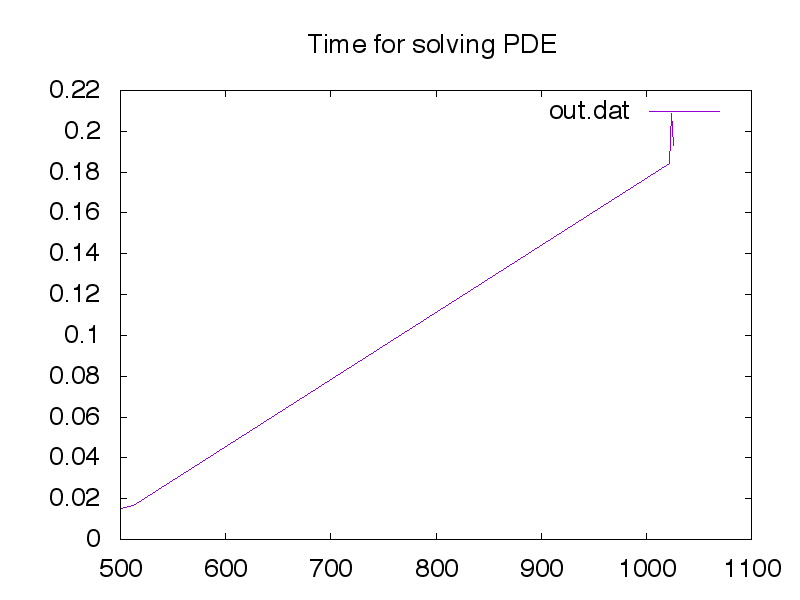
\includegraphics[width=90mm]{oldtime.png}
		\caption{Tempo para N\{x,y\} = \{500, 512, 1022, 1024, 1026\} no programa original}
	\end{figure}
	
	\newpage

% ------------------------------------------------------ %
\section{Análise de Funções}

	\subsection{Cálculo do Número de Operações\\ em Ponto Flutuante}
		Para obtermos a função $FLOPS$ de cada versão do programa, simplesmente contamos o número de operações em ponto flutuante realizadas dentro do laço principal da função analisada (Gauss-Seidel ou cálculo do resíduo) e multiplicamos esse número pela quantidade de vezes que o laço é executado: $(n_x + 1)\times(n_y + 1)$.
		\subsubsection{Método de Gauss-Seidel}
		\begin{align*}
			FLOPS(n_x,n_y) &= 8\times(n_x+1)\times(n_y+1)
		\end{align*}
		\subsubsection{Cálculo do Resíduo}
		\begin{align*}
			FLOPS(n_x,n_y) &= 2\times(n_x+1)\times(n_y+1)\times(2\times(ny+1)+1)
		\end{align*}
			
	\subsection{Cálculo da Quantidade de Memória Utilizada}
		Para obtermos a quantidade de memória utilizada, bastou somar os tamanhos dos vetores utilizados e multiplicar o resultado por 8, que é o tamanho em bytes do tipo \texttt{double} em C.
		\begin{align*}
			MEM(n_x,n_y) &= ((n_x+1)\times(n_y+1)\times(2\times(ny+1)+1)+3\times(n_x+1)\times(n_y+1))\times 8bytes
		\end{align*}
		

	\newpage
	\subsection{Gráficos de Desempenho}
		\subsubsection{Método de Gauss-Seidel}
		\begin{figure}[ht!]
			\centering
			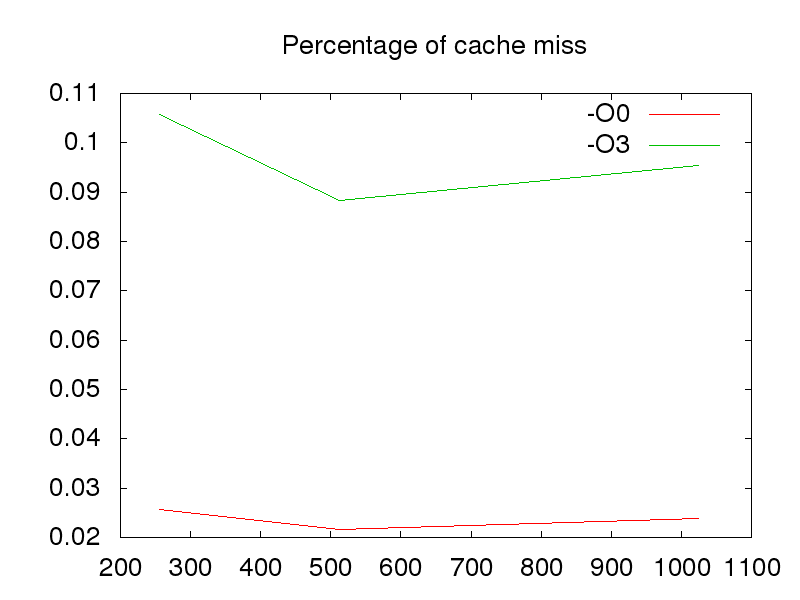
\includegraphics[width=90mm]{old_gs_cache.png}
			\caption{Porcentagem de cache misses para N\{x,y\} = \{256, 512, 1024\} no programa original}
		\end{figure}

		\begin{figure}[ht!]
			\centering
			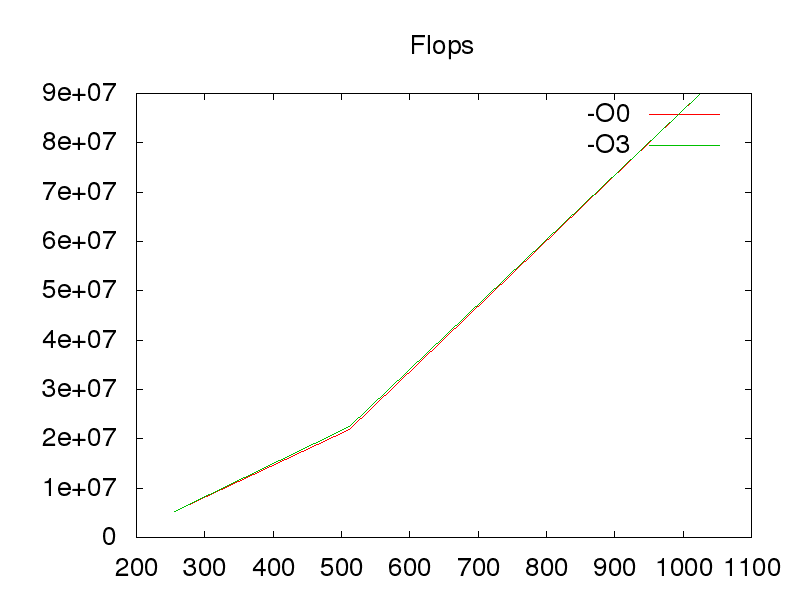
\includegraphics[width=90mm]{old_gs_flops.png}
			\caption{Número de operações em ponto flutante para N\{x,y\} = \{256, 512, 1024\} no programa original}
		\end{figure}
		
		\newpage
		\begin{figure}[ht!]
			\centering
			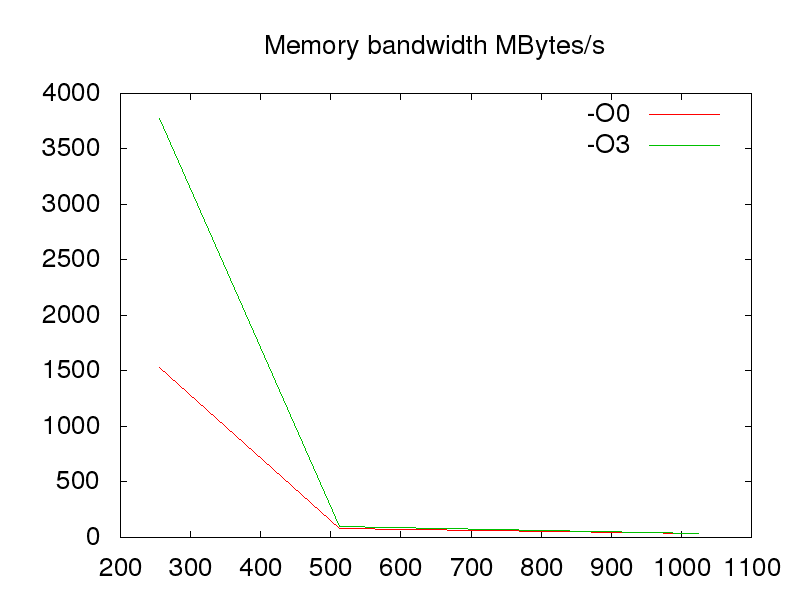
\includegraphics[width=90mm]{old_gs_mem.png}
			\caption{Banda de memória para N\{x,y\} = \{256, 512, 1024\} no programa original}
		\end{figure}
		
		\newpage
		\subsubsection{Cálculo do Resíduo}
		\begin{figure}[ht!]
			\centering
			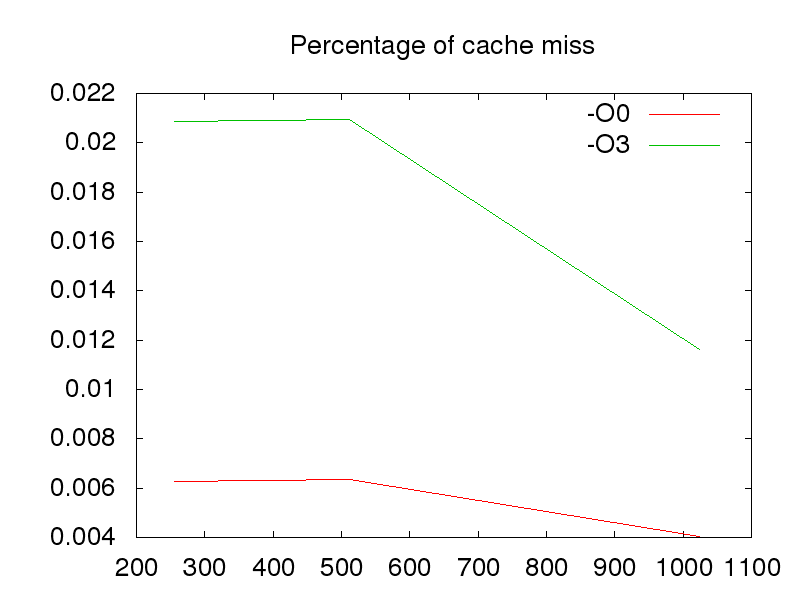
\includegraphics[width=90mm]{old_res_cache.png}
			\caption{Porcentagem de cache misses para N\{x,y\} = \{256, 512, 1024\} no programa original}
		\end{figure}
		
		\begin{figure}[ht!]
			\centering
			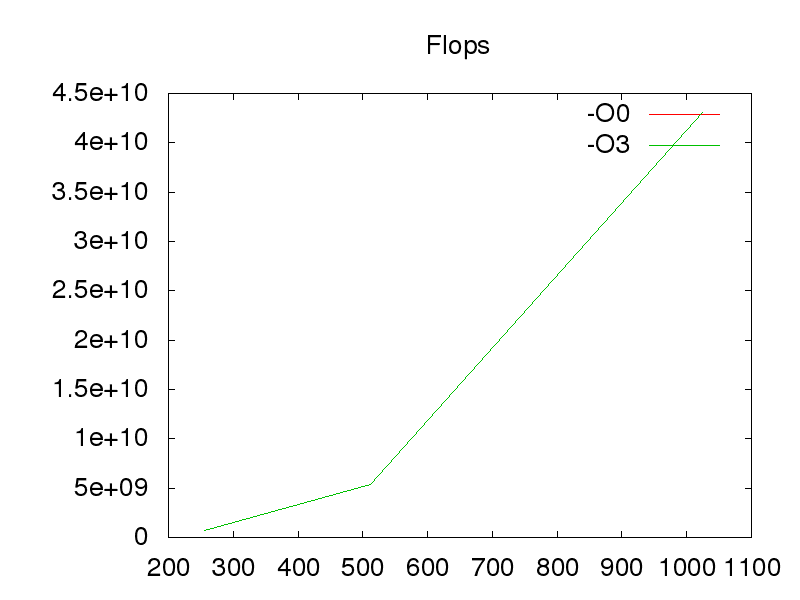
\includegraphics[width=90mm]{old_res_flops.png}
			\caption{Número de operações em ponto flutuante para N\{x,y\} = \{256, 512, 1024\} no programa original}
		\end{figure}

		\newpage
		\begin{figure}[ht!]
			\centering
			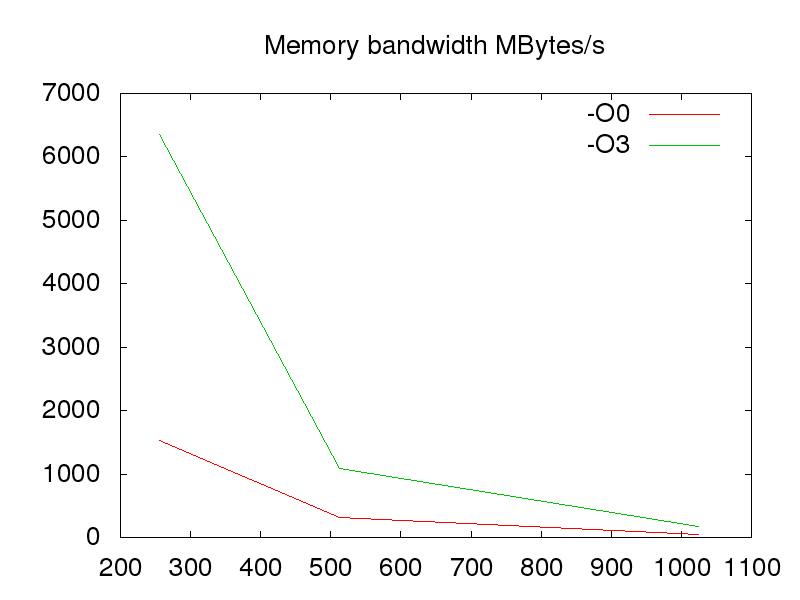
\includegraphics[width=90mm]{old_res_mem.png}
			\caption{Banda de memória para N\{x,y\} = \{256, 512, 1024\} no programa original}
		\end{figure}
	\newpage
		
	\subsection{Análise dos Dados}
	
	Nos gráficos que mostram a porcentagem de \emph{cache misses}, é visível que o número é muito maior no cálculo de Gauss-Seidel do que no cálculo do resíduo.
	Isso se deve aos quatro desvios presentes no laço que calcula Gauss-Seidel, enquanto o cálculo do resíduo carece de desvios.
	Além disso, há uma notável diminuição na porcentagem de \emph{cache misses} no cálculo do resíduo para uma discretização de 1024 comparada a uma de 512.
	É possível que os números absoluto de \emph{cache misses} nas duas execuções sejam similares, mas são proporcionalmente diferentes comparados ao número da discretização.
	
	O cálculo do resíduo efetua muito mais operações em ponto flutuante que o cálculo de Gauss-Seidel, porque percorre uma dimensão a mais do vetor A.
	Então, sua complexidade está na ordem de $O(n^3)$.
	
	Também é notável que as execuções utilizando otimização O3 sofrem de mais \emph{cache misses} e usam mais banda de memória, mas as quantidades de operações em ponto flutuante permanecem quase idênticas às das execuções sem otimização (usando O0). 
	
\newpage

% ------------------------------------------------------ %
\section{Otimização do Ponto de Interesse}

O ponto de interesse escolhido foi o cálculo do vetor $x$ no método de Gauss-Seidel.
Para isso, otimizações foram feitas nas estruturas de dados usadas durante o cálculo e na estrutura do laço em si.

	\subsection{Estrutura de dados}
	A estrutura de dados que mais sofreu alterações foi a matriz $A$.
	Na versão original do programa, $A$ tinha o tamanho de $((n_x+1)\times(n_y+1))^2$, representando a matriz inteira do método analítico de Gauss Seidel.
	
	Olhando para a matriz $A$, percebemos que grande parte das posições tinham valor $0$ e que os valores de interesse de cada linha estavam numa distância de $(n_y+1)$ da diagonal principal da matriz.
	Ou seja, os dados que estavam além desse intervalo eram sempre $0$ e poderiam ser ignorados.
	
	Além disso, percebemos que as posições ao redor da diagonal principal sempre seguiam o seguinte padrão:
	
	\begin{center}
		\texttt{$h_x$ 0 ... 0 $h_y$ 1 $h_y$ 0 ... 0 $h_x$}
	\end{center}
	
	Onde o elemento na diagonal principal é sempre $1$, $h_x$ e $h_y$ representam a dependência dos pontos adjacentes, o número de zeros varia de acordo com $n_y$.
	Sendo assim, podíamos ignorar as posições que sempre continham $1$ ou $0$, além de evitar a repetição de $h_x$ e $h_y$.
	
	Também foi possível ver que os valores de $h_x$ e $h_y$ permaneciam constantes em quase todas as linhas da matriz, exceto nas linhas em que não estavam presentes.
	As linhas que não continham $h_x$ e $h_y$ representavam os pontos das bordas da grade, que são calculadas separadamente.
	Logo, foi possível ver que uma matriz que simplesmente nos dizia se um determinado ponto é ou não uma borda era suficiente para fazer os cálculos de Gauss-Seidel, se salvássemos $h_x$ e $h_y$ em variáveis separadas.
	
	Portanto, a matriz $A$ passou a ter o tamanho de $(n_x+1)\times(n_y+1)$ e utiliza o tipo de dados \emph{short int}, pois apenas armazenamos $0$ quando o ponto é uma borda ou $1$ caso contrário.
	
	Após isso, percebemos que não havia necessidade de armazenar essas informações em um vetor de qualquer maneira.
	Assim, modificamos o laço do Gauss-Seidel para que percorra apenas as posições relevantes de $x$ e $B$ (que correspondem aos pontos que não são bordas).
	Dessa forma, é possível evitar condições durante o laço, pois os elementos de $x$ correspondentes a posições de borda serão $0$ e, na multiplicação, tornarão os valores a serem desconsiderados em $0$ também.
	
	Na versão nova do programa, então, não há qualquer representação para a matriz A, e essa parte do problema foi resolvida de forma algébrica.

	\subsection{Código}
	
	Na versão anterior do programa, o laço de Gauss-Seidel continha quatro desvios condicionais, um para cada borda.
	Nesta versão, não temos mais desvios porque, se o resultado de uma operação deve ser desconsiderado, essa operação resultará em $0$.
	
	Quatro operações são realizadas utilizando os valores de $h_x$ e $h_y$ e outras posições do vetor $x$ (que são $0$ se representa um ponto de borda).
	Na versão original do programa, as quatro operações eram armazenadas na variável \texttt{temp} utilizando o operador \texttt{+=}.
	Isso causava problemas no pipeline da execução, pois gerava uma dependência de dados onde todas as operações em ponto flutuante da linha anterior precisavam ser computadas antes do início dos cálculos da próxima.
	Agora, as quatro operações são salvas em variáveis separadas para permitir melhor uso do pipeline. 
	Essas quatro variáveis são então computadas após as quatro operações.
	
	Adicionalmente, utilizamos a técnica de \emph{loop unrolling} de passo 2 para melhorar ainda mais o desempenho do programa.
	Ao invés de quatro operações principais, cada iteração do laço agora faz oito operações.
	Experimentamos aumentar o passo do \emph{unroll} para 4, mas a diferença no tempo de execução foi irrisória e optamos por continuar utilizando passo 2 para manter a legibilidade do código.
	
	Todas otimizações foram replicadas no laço que calcula o resíduo do método de Gauss-Seidel e obtivemos melhoras semelhantes de desempenho.

\newpage

% ------------------------------------------------------ %
% Resultados %
\section{Resultados}

	\subsection{Limite Superior da Discretização}

	\begin{align*}
		T &\cong n_x + 1 = n_y + 1 \\
		|X| &= (n_x+1)\times(n_y+1)\times8 bytes \cong T^2\times8 bytes \\
		|B| &= (n_x+1)\times(n_y+1)\times8 bytes \cong T^2\times8 bytes \\
		|R| &= (n_x+1)\times(n_y+1)\times8 bytes \cong T^2\times8 bytes \\
		|X| + |B| + |R| &= 24000000000 \\
		3\times T^2\times8 &= 24000000000 \\
		T^2 &= 1000000000\\
		T &\cong 31622
	\end{align*}

	A nova versão do programa aceita valores de até aproximadamente 31.621 para $n_y$ e $n_x$ numa máquina com 24GB de 	RAM e desconsiderando o uso de memória virtual e qualquer outro uso de memória que seja necessário.
	%Ou seja, pode computar até 54.756 de pontos.
	
	%Apesar do programa original ser um desastre, o novo programa é razoável, mas mesmo assim uma bosta. Sabe porque? por causa da porra da alemanha chamada likwid! caralho.
	
	\subsection{Tempo de Execução}
	\begin{figure}[ht!]
		\centering
		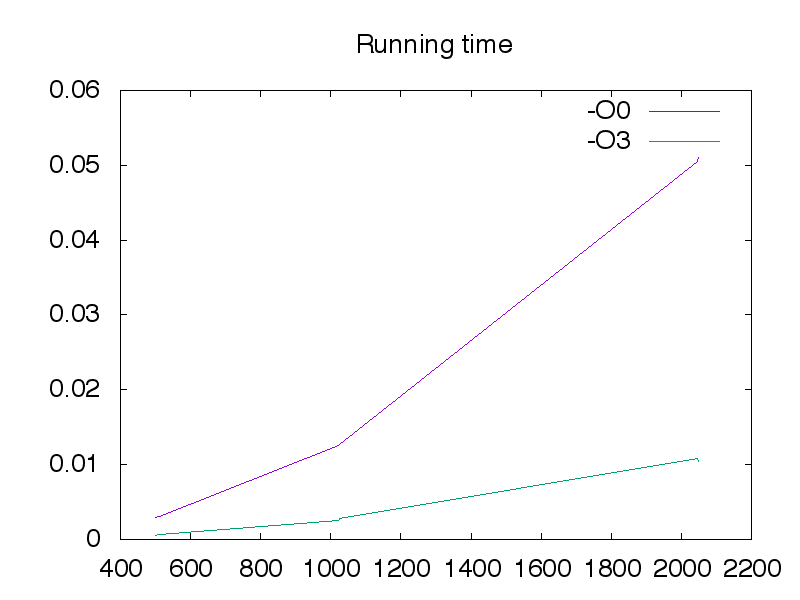
\includegraphics[width=90mm]{newtime.png}
		\caption{Tempo para N\{x,y\} = \{500, 512, 1022, 1024, 1026, 2046, 2048\} no novo programa}
	\end{figure}


	\subsection{Cálculo do Número de Operações\\ em Ponto Flutuante}
		\subsubsection{Método de Gauss-Seidel}
		\begin{align*}
			FLOPS(n_x,n_y) &= 8\times n_x\times n_y
		\end{align*}
		\subsubsection{Cálculo do Resíduo}
		\begin{align*}
			FLOPS(n_x,n_y) &= 9\times n_x\times n_y
		\end{align*}

	\subsection{Cálculo da Quantidade de Memória Utilizada}
		\begin{align*}
			MEM(n_x,n_y) &= 3\times(n_x+1)\times(n_y+1)\times 8bytes
		\end{align*}

	\newpage
	\subsection{Gráficos de Desempenho}
		\subsubsection{Método de Gauss-Seidel}
		\begin{figure}[ht!]
			\centering
			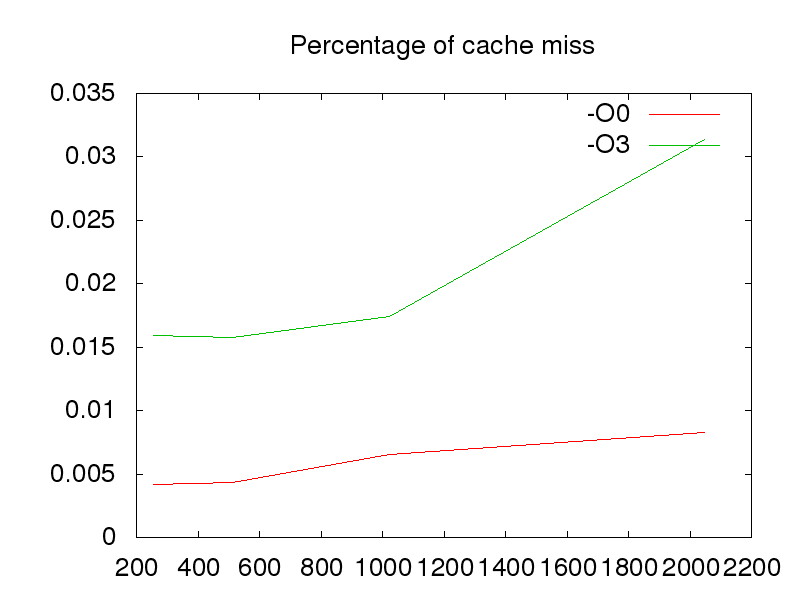
\includegraphics[width=90mm]{new_gs_cache.png}
			\caption{Cache misses para N\{x,y\} = \{256, 512, 1024, 2048\} no novo programa}
		\end{figure}
		
		\begin{figure}[ht!]
			\centering
			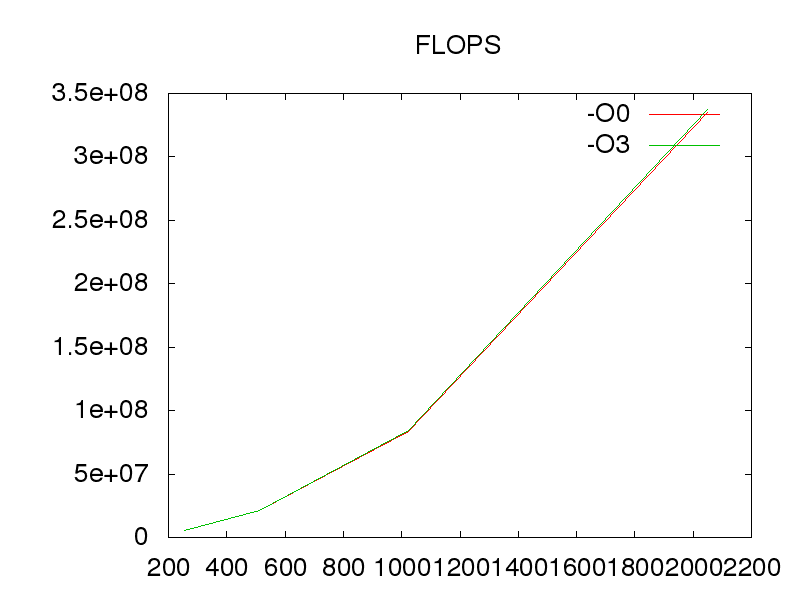
\includegraphics[width=90mm]{new_gs_flops.png}
			\caption{Número de operações em ponto flutante N\{x,y\} = \{256, 512, 1024, 2048\} no novo programa}
		\end{figure}
		
		\newpage
		\begin{figure}[ht!]
			\centering
			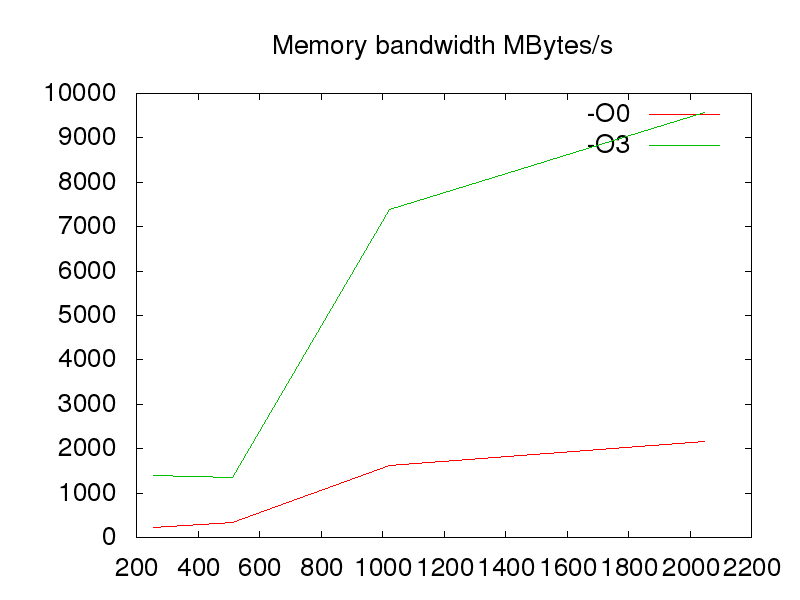
\includegraphics[width=90mm]{new_gs_mem.png}
			\caption{Banda de memória para N\{x,y\} = \{256, 512, 1024, 2048\} no novo programa}
		\end{figure}
		
		\newpage
		\subsubsection{Cálculo do Resíduo}
		\begin{figure}[ht!]
			\centering
			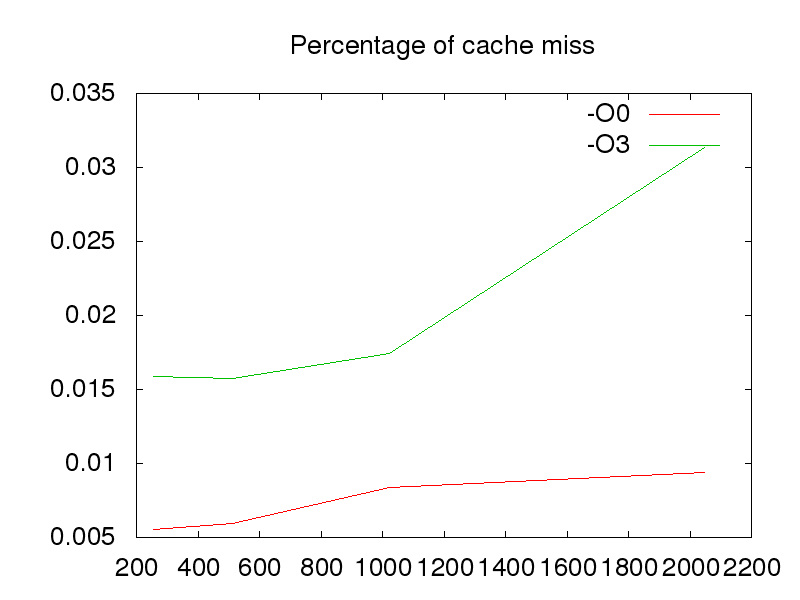
\includegraphics[width=90mm]{new_res_cache.png}
			\caption{Cache misses para N\{x,y\} = \{256, 512, 1024, 2048\} no novo programa}
		\end{figure}
		
		\begin{figure}[ht!]
			\centering
			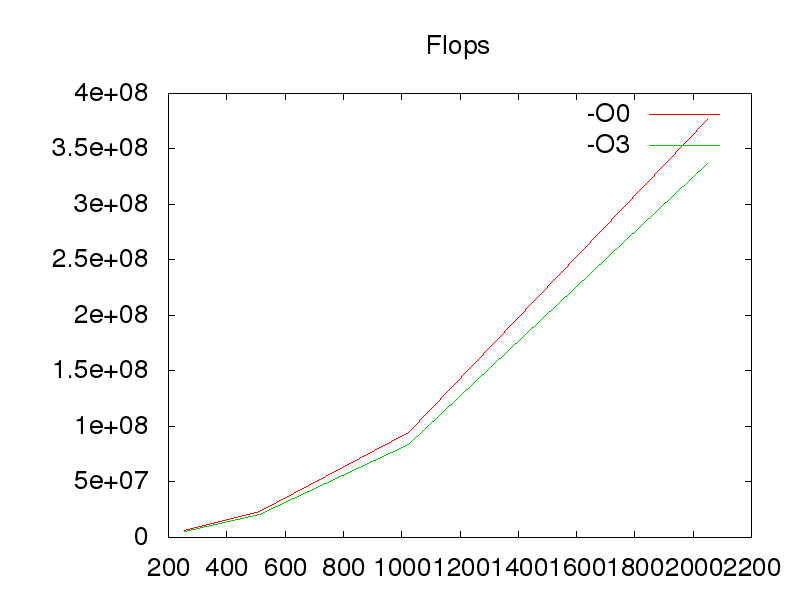
\includegraphics[width=90mm]{new_res_flops.png}
			\caption{Número de operações em ponto flutante N\{x,y\} = \{256, 512, 1024, 2048\}}
		\end{figure}
		
		\newpage
		\begin{figure}[ht!]
			\centering
			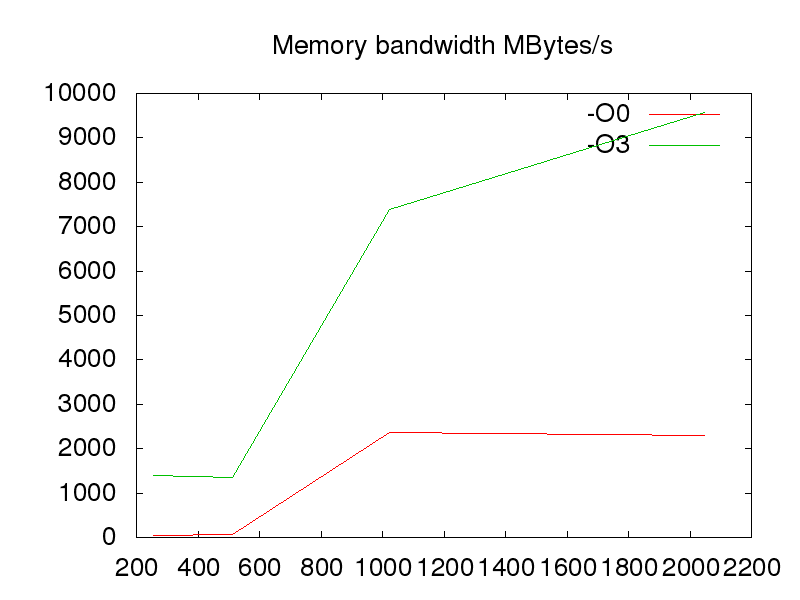
\includegraphics[width=90mm]{new_res_mem.png}
			\caption{Banda de memória para N\{x,y\} = \{256, 512, 1024, 2048\} no novo programa}
		\end{figure}
		\newpage
		
	\subsection{Conclusões}
	Como pode ser visto nos gráficos, a nova versão do programa tem muitas melhoras de performance em relação ao original.
	
	O tempo de execução para uma discretização de 2048, por exemplo, está uma ordem de grandeza menor que para uma discretização de 1024 (e executando tempo ainda menor que uma discretização de 512) no programa antigo.
	
	O número de operações em ponto flutuante no cálculo do Gauss-Seidel sofreu uma alteração pequena, mas, em compensação, houve uma diminuição dramática no número de operações no cálculo do resíduo, com valores reduzidos em duas ordens de grandeza.
	
	A porcentagem de \emph{cache misses} no cálculo do Gauss-Seidel também caiu em duas ordens de grandeza nas execuções sem otimizações, mas não mudou muito no cálculo dos resíduos.

	A banda de memória aumentou bastante na nova versão, tanto no Gauss-Seidel quanto no resíduo, que acontece porque o programa novo executa em muito menos tempo que o original, fazendo com que a memória seja acessada mais vezes por segundo.Além disso, há menos memória a ser acessada e é acessada mais constantemente devido à remoção dos desvios condicionais durante o laço.
	
\end{document}